\if0
\section{高速化の方針}
\fi
\section{A Policy of Speeding up}

\if0
高速化の方針として逐次プログラミングにおける最適化と並列化の両方を考える.
\fi
I consider both optimizations in sequential programming and parallelization
as a policy of fast methods.

\if0
\section{逐次プログラムにおける高速化手法}
\fi
\section{Fast methods in sequential program}

\if0
\subsection{データ変更の有無による条件分岐の除去 \label{sss:no_set}}
\fi
\subsection{Removal of conditional branch for data update} \label{sss:no_set}


\if0
\figref{src:reg} に示した実装では,reg クラスのインスタンスの値を更新する方法としてブロッキング代入とノン・ブロッキング代入の 2 つが存在する.
\fi
In the implementation shown \figref{src:reg},
ArchHDL gives non-blocking assignment and blocking assignment as methods of updating the value of the \textit{reg} class instance.

\if0
ブロッキング代入について考える.reg クラスのインスタンスにブロッキング代入が行われた時に curr\_ の値を書き換える.
\fi
I consider blocking assignment.
The member variable \textit{curr\_} of the \textit{reg} class instance must be assigned to the value
if the blocking assignment is carried out to the \textit{reg} class instance.

\if0
一方でノン・ブロッキング代入について考える.
reg クラスのインスタンスにノン・ブロッキング代入が行われた時にメンバ変数 set\_ を true にし,メンバ変数 next\_ に値を代入する.
そして reg::Update 内では set\_ が true の時だけ next\_ をメンバ変数 curr\_ に代入する.
これは reg クラスのインスタンスの値を変更したサイクルのみで,
その reg クラスのインスタンスの値を次サイクルに移る前に新しい値に更新することを意味する.
\fi
I consider non-blocking assignment.
The member variable \textit{set\_} of the \textit{reg} class instance is assigned to true
and the member variable \textit{next\_} is assigned to the value
if the non-blocking assignment is carried out to the \textit{reg} class instance.
Only when the member variable \textit{set\_} is true, the member variable \textit{next\_} is assigned to the value of the member variable \textit{curr\_} in the \textit{Update} function which is a member method of \textit{reg} class.
It shows the value of the register is updated to the new value before the only cycle which is the non-blocking assignment is carried out to the \textit{reg} class instance.

\if0
\figref{src:reg} に示した実装では,
更新されない reg クラスのインスタンスの curr\_ と next\_ の値が同じであるため,代入する処理を行う必要はない.
よって set\_ 変数を用いて不要な代入を避けている.
reg クラスのインスタンスの更新頻度が低い回路であればこの実装が効率的である.
\fi
In the implementation shown \figref{src:reg},
it is not necessary to perform the process of assignment
if the values of the \textit{next\_} and \textit{curr\_} of the \textit{reg} class instance are same.
Therefore the unnecessary assignment is avoided using the variable \textit{set\_}.
This implementation may be effective if the \textit{reg} class instance is rarely updated.

\if0
提案手法について述べる.
この set\_ 変数が true の時のみ代入するのではなく,
次サイクルに移る前に next\_ の値を curr\_ に常に代入するようにする.
こうすることによって分岐のオーバーヘッドが無くなるため,ノン・ブロッキング代入が頻繁に行われる回路で速度向上が期待できる.
\fi
I describe the proposed method.
The value of the \textit{next\_} is always assigned to the variable \textit{curr\_} every cycle.
It eliminates without the overhead of the \textit{if} branch.
This implementation is effective if the \textit{reg} class instance is updated frequently.

% SWoPP より追加

\begin{figure}[tb]
 \lstinputlisting[language=c++]{src/reg_no_set.cc}
\if0
 \caption{条件分岐を除去した reg クラス}
\fi
 \caption{The source code of \textit{reg} class which is removed of the conditional branch}
 \label{src:reg_no_set}
\end{figure}

\if0
\figref{src:reg_no_set} に提案手法の実装を示す.
\figref{src:reg} の実装から set\_ 変数を除いている.
\fi
\figref{src:reg_no_set} shows the implementation of the proposed method.
It is removed of the variable \textit{set\_} from the implementation shown \figref{src:reg}.

% 追加ここまで


\if0
\subsection{値を配列として格納しメモリ配置を工夫} \label{sss:mem_copy}
\fi
\subsection{Storing register values to the continuous memory location} \label{sss:mem_copy}

\begin{figure}[t]
 \centering
 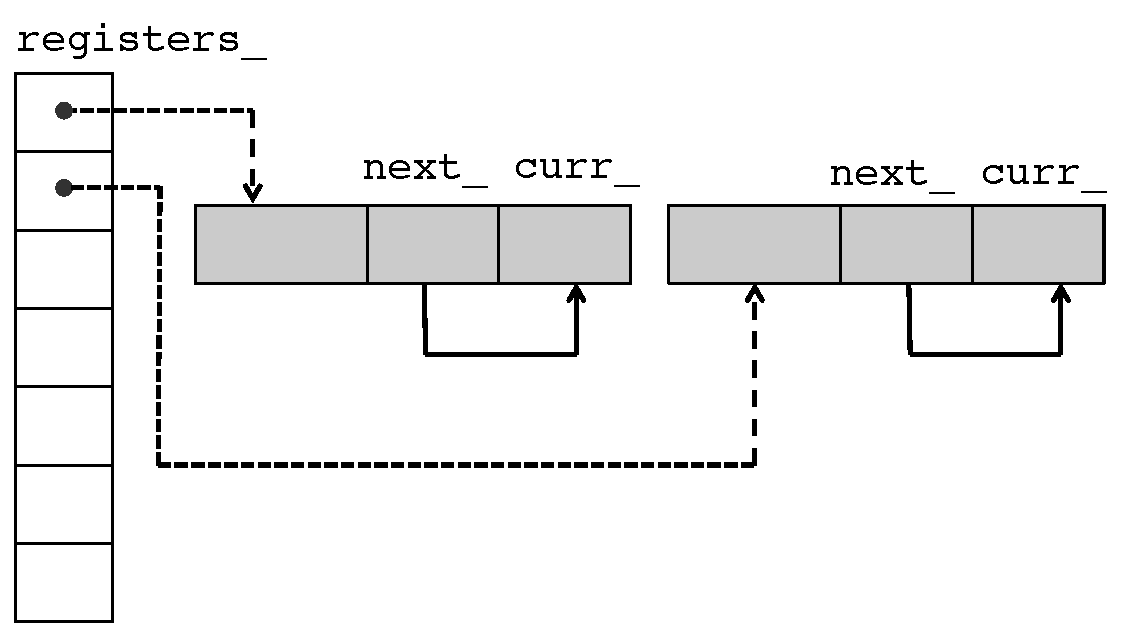
\includegraphics[clip,width=\linewidth-30pt]{registers_orig}
\if0
 \caption{ArchHDL における reg クラスのインスタンスの処理の様子}
\fi
 \caption{The process of the \textit{reg} class instance with ArchHDL}
 \label{fig:regs}
\end{figure}

\if0
\figref{fig:regs} は ArchHDL における reg クラスのインスタンスの処理の様子である.
\figref{src:class_singleton} の 44 行から 46 行の処理を表している.
reg クラスのインスタンスが灰色に塗られており,左からクラスのメタデータ,next\_, curr\_ を表している.
左側の大きな枠が\figref{src:class_singleton} の 18 行の \verb`std::vector` 型の registers\_ である.
実線矢印は代入を表し.点線矢印はポインタ参照を表す.
\fi
\figref{fig:regs} shows the process of the \textit{reg} class instance with ArchHDL.
It denotes \figref{src:class_singleton} from the 44th line to the 46th line.
The \textit{reg} class instances are painted gray
and metadata of the class, the variable \textit{next\_} and the variable \textit{curr\_} are represented from the left.
Big frame on the left denotes \textit{registers\_} of \verb`std::vector` in the 18th line of \figref{src:class_singleton}.
Solid arrows represent an assignment.
Dotted arrows represent a pointer reference.

\if0
ArchHDL ではノン・ブロッキング代入をシミュレーションするために registers\_ の値を上から順に辿り,
reg クラスの各インスタンスのポインタを取得する.
そして reg クラスの全インスタンスの reg::Update() メソッドを呼ぶ.
\fi
To simulate the non-blocking assignment in ArchHDL,
it follows the values of the \textit{registers\_}
and obtains a pointer to the \textit{reg} class instances.
The \textit{Update} method of the \textit{reg} class instances is called.

\if0
\ref{sss:no_set} 節で述べたデータ変更の有無による条件分岐の除去を行うと reg::Update() メソッド内で行なっている
reg クラスのインスタンスの curr\_ に next\_ の値を代入する処理は
毎サイクル全 reg クラスのインスタンスで実行されることになる.
\fi
If I implement the removal of conditional branch by the presence or absence of data changes described in Section \ref{sss:no_set},
the value of the \textit{next\_} is always assigned to the variable \textit{curr\_} every cycle in \textit{reg::Update} method.

\if0
この代入する処理と reg::Update() メソッドの関数呼び出しの 2 つのオーバーヘッドが ArchHDL の高速化を妨げている.
\fi
The two overheads of this assignment and function call make the speed of the ArchHDL slow down.

\begin{figure}[t]
 \centering
 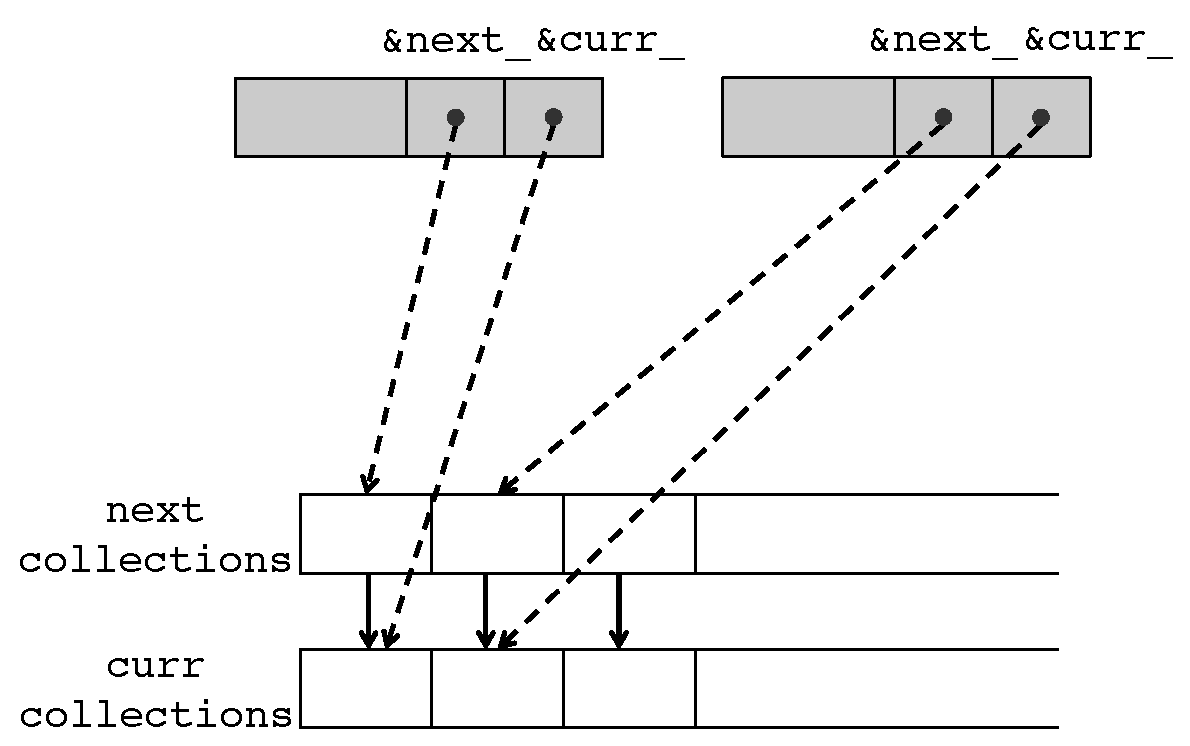
\includegraphics[clip,width=\linewidth-30pt]{registers_mem}
\if0
 \caption{値を配列として格納しメモリ配置を工夫した reg クラスのインスタンスの処理の様子}
\fi
 \caption{The process of the \textit{reg} class instance stored as an array}
 \label{fig:mem_copy}
\end{figure}

\if0
提案手法について述べる.
\figref{fig:mem_copy} に値を配列として格納しメモリ配置を工夫した reg クラスのインスタンスの処理の様子を示す.
\figref{fig:mem_copy} は提案手法である.
提案手法では全 reg クラスのインスタンスは現在の値と次サイクルの値の実体は持たず,ポインタを保持するように変更している.
\fi
I describe the proposed method.
\figref{fig:mem_copy} shows the process of the \textit{reg} class instance stored as an array.
\figref{fig:mem_copy} shows the proposed method.
That all of the \textit{reg} class instances have the value of the next cycle and the current value is changed into holding each pointer in the proposed method.
\if0
reg クラスのインスタンスが灰色に塗られており,左からクラスのメタデータ,\&next\_, \&curr\_ を表している.
\&next\_, \&curr\_ は next\_, curr\_ のポインタである.
下の枠が next\_, curr\_ の値をまとめた配列であり,
ここでは next collections, curr collections と呼ぶ.
実線矢印は代入を表し,点線矢印はポインタの参照先を表す.
\fi
The \textit{reg} class instances are painted gray
and metadata of the class, the \texttt{\&next\_} and the \texttt{\&curr\_} are represented from the left.
The \texttt{\&next\_} and the \texttt{\&curr\_} is a pointer of \textit{next\_} and \textit{curr\_}.
Big frames on the bottom denote the arrays which summarize the value of \textit{next\_} and \textit{curr\_}.
The next collections and the curr collections is named here.
Solid arrows represent an assignment.
Dotted arrows represent a pointer reference.

\if0
ArchHDL の実装では次サイクルに移る前に行われる curr\_ に next\_ の値を代入する処理は
reg クラスのインスタンスが存在するアドレスを調べる必要がある.
しかし値を配列として格納しメモリ配置を工夫すると\figref{fig:mem_copy} に示すように単純な代入となる.
また今まで飛び飛びのアドレスに格納されていた next\_ と curr\_ のメモリ配置がまとまるのでメモリアクセスが連続的に行える.
さらに reg::Update() の関数呼び出しが不要となり,関数呼び出しのオーバーヘッドもなくなる.
これらの理由により高速化が期待できる.
\fi
It is necessary to examine the address the \textit{reg} class instances exist in the implementation of original ArchHDL
before the process of assigning the value of the \textit{next\_} to the variable \textit{curr\_} is executed before moving the next cycle.
But if the implementation of \textit{reg} class is devised a memory allocation and stored as an array, \textit{Update} method is a simple assignment as shown in \figref{fig:mem_copy}.
Memory access can be carried out continuously
because the memory allocation of the variable \textit{next\_} and \textit{curr\_} is continuous.
The memory allocation is discrete in the implementation of original ArchHDL.
The overhead of a function call is eliminated
because it is unnecessary to call the \textit{Update} method.
In the above reasons, speeding up can be expected.

\if0
提案手法の実装について述べる.
next collections, curr collections として 2 つの十分大きな \verb/unsigned int/ 型の配列を用意する.
記述された型に応じて,reg クラスのコンストラクタが next\_, curr\_ それぞれの領域を next collections, curr collections に確保する.
確保する領域は参照の高速化のために 4 バイトの倍数とする.
確保された next\_ と curr\_ のアドレスを取得し,インスタンス内の \&next\_, \&curr\_ がそれを保持する.
これまで reg クラスの全インスタンスの reg::Update() メソッドを呼び出していたところを next\_ collections から curr\_ collections の値コピーに変更する.
\fi
I describe the implementation of the proposed method.
2 large arrays of the type of \verb/unsigned int/ are allocated as the next collections and the curr collections.
Depending on the type of the template arguments, the constructor of \textit{reg} class allocates each region to the next collections and the curr collections.
The allocated region is a multiple of 4 bytes to speed up reference.
The addresses of the variable \textit{next\_} and \textit{curr\_} are acquired and
the \texttt{\&next\_} and the \texttt{\&curr\_} hold them.
The \texttt{reg::Update} method is not called
but the next collections are assigned to the curr collections.


\if0
\subsection{ダブルバッファリング}

これまでの実装では \ref{ss:implementation} 章で述べたように
reg クラスのインスタンスの次サイクルの値が次サイクルに移る前に reg クラスのインスタンスの現在の値に代入される.
そこで偶数回目の実行と奇数回目の実行で次サイクルの値と現在の値を格納している変数をを入れ替えれば
(ダブルバッファリング)代入が減ることが期待できる.

\begin{figure}[t]
 \begin{center}
  \input{img/reg_curr_next}
 \end{center}
 \caption{reg クラスのインスタンスの変数保持の処理の様子}
 \label{fig:reg_curr_next}
\end{figure}

\begin{figure}[t]
 \begin{center}
  \input{img/double_buffer2}
 \end{center}
 \caption{ダブルバッファリングの処理の様子}
 \label{fig:double_buffer}
\end{figure}

\figref{fig:reg_curr_next} はこれまでの ArchHDL の reg クラスのインスタンスの値の保持のイメージである.
読み込み用と書き込み用の変数をそれぞれ保持している.
読み込み用が現在の値であり,書き込み用が次サイクルの値である,
次サイクルに移る前に書き込み用の値が読み込み用の変数に書き込まれる.

\figref{fig:double_buffer}
はダブルバッファリングのイメージである.
奇数回目のサイクルと偶数回目のサイクルで読み込み用と書き込み用の変数を入れ替える.
これにより奇数回目のサイクルで書き込み用であった変数には値が書き込まれているので次サイクルの偶数回目のサイクルで読み込み用として使用出来る.
これを繰り返すことで,次サイクルに移る前に行われる代入処理を無くせる.

しかし今回の手法では reg クラスのインスタンスへ値の書き込みが行われなかった場合に
reg クラスのインスタンスのその時の書き込み用の値に更新が入らない.
次サイクルではその書き込み用の値がそのまま現在の値として使用されるので古い値が使われてしまう.
そのため単純に入れ替えるだけの実装では誤ったシミュレーションを行なってしまう.

また今回の手法はサイクルの回数で依存関係が発生するので \ref{ss:parallel} 節で述べる並列化ができない.

よってライブラリの実装として導入するのは困難であるが,
reg クラスのインスタンスへ常に書き込みが行われるカウンタ回路で試したところ効果があった(具体的な数字).
常に reg クラスのインスタンスに書き込みが行われるハードウェアシミュレーションを逐次処理で行いたい場合には高い効果が期待できる.

以上の理由から本論文ではダブルバッファリングによる評価は行わない.

\fi

\if0
\section{並列化による高速化} \label{ss:parallel}
\fi
\section{The parallelization of the execution of multiple instances} \label{ss:parallel}

\if0
これまで逐次プログラミングにおける高速化を考えてきたが,本節では並列化による高速化について考える.
\fi
I have been considering the fast methods in sequential programming,
however I consider the speed up by parallelization in this section.

\if0
\figref{src:class_singleton} の 40 行〜 47 行に示すように
毎サイクル,Module クラスと reg クラスの全インスタンスの Module::Always() メソッドと reg::Update() メソッドが呼び出されている.
\fi
As \figref{src:class_singleton} is shown from the 40th line to the 47th line,
all of the \textit{Module} and \textit{reg} class instances
call \textit{Module::Always} and \textit{reg::Update} method every cycle.

\if0
\figref{src:class_singleton} の41行〜43行で実行される Module::Always() メソッドはユーザが自由に記述できる.
そのため各 Module クラスのインスタンスで独立に Module::Always() メソッドが実行できる保証はない.
しかしここでは独立に実行できると仮定する.
独立に実行できる条件は今後の研究課題とする.
この場合\figref{src:class_singleton} の41行〜43行に示している Module::Always() メソッドの実行は並列化が可能である.
\fi
From the 41th line to the 43th line in \figref{src:class_singleton},
\textit{Module::Always} method can be described freely by the user.
Therefore there is no guarantee that \textit{Module::Always} method can be executed separately for each of the \textit{Module} class instances.
However, it is assumed that it can execute independently here.
It is a special challenge for the future conditions.
It is possible to parallelize the execution of the \textit{Module::Always} method.

\if0
\figref{src:class_singleton} の 44 行〜 46 行で行われるレジスタの更新は\figref{fig:regs} の実線で表されている.
各インスタンスで独立に行えるので並列化が可能である.
\fi
\figref{fig:regs} shows the update of the register by solid arrows.
It is possible to execute independently for each instance.
It is possible to parallelize the execution of the \textit{reg::Update} method.

\if0
\figref{src:class_singleton} の41行〜47行に示している Module クラスと reg クラスの全インスタンスの Module::Always() メソッドと reg::Update() メソッドの実行は並列化が可能である.
提案手法について述べる.この部分を並列化する.並列化には OpenMP~\cite{openmp} を用いる.
\fi
I describe the proposed method.
I parallelize \textit{Module::Always} and \textit{reg::Update} method from the 41th line to the 43th line in \figref{src:class_singleton}.
I use OpenMP~\cite{openmp} to parallelize.

\begin{figure}[t]
 \lstinputlisting[language=c++]{src/exec_openmp.cc}
\if0
 \caption{Exec メソッド内の for 文を OpenMP で並列化したプログラム}
\fi
 \caption{The source code which is parallelized in the \textit{for} statements of \textit{Exec} method with OpenMP in 8 threads}
 \label{src:exec_openmp}
\end{figure}

\if0
\figref{src:exec_openmp} は\figref{src:class_singleton} の 40 行〜 47 行が 8 スレッドで並列化が行われるように OpenMP 指示文を与えたソースコードである.
2 行目は並列化を何スレッドで行うかを与えている.
今回は 8 をスレッド数に指定している.この数字は環境によって変えることができる.
4 行目と 8 行目は for 文の実行を並列化する OpenMP 指示文である.
\fi
\figref{src:exec_openmp} is an improvement on \figref{src:class_singleton} from the 40th line to the 47th line.
\figref{src:exec_openmp} shows the source code which is parallelized in the \textit{for} statements of \textit{Exec} method with OpenMP in 8 threads.
The number of threads can be changed by the environment.
The 2nd line of \figref{src:exec_openmp} give parallelization in 8 threads.
The 4th line and the 8th line are OpenMP directives to parallelize the execution of the \textit{for} statement.

\if0
一般に,並列化を行う場合は各スレッドに対して均等に負荷を与えることが重要である.
OpenMP では for 文の負荷を分散するスケジュール方法として,静的に決定する static や,動的に決定する dynamic など複数の方法が存在する.
一般に,スケジュール方法に dynamic を指定した場合,各スレッドに割り当てられる負荷が均等に近くなるメリットはあるが,オーバーヘッドが大きいデメリットがある.
ArchHDL により記述されたハードウェア記述では各モジュールと各レジスタの負荷が大幅に変わらないのであれば,static を指定した方が効率が良いと考えられる.
\fi
Generally, it is important that parallelization divide the task equally to each thread.
Several methods such as \textit{static} to determine statically
and \textit{dynamic} to determine dynamic exist
as a way to balance the load of the \textit{for} statement in OpenMP.
If you specify the \textit{dynamic} as a way to schedule,
it has an advantage as a load assigned to each thread is almost equal
but a disadvantage as large overhead.
If load of each register and each module is not very difference in the hardware description in ArchHDL,
it is considered desirable to specify \textit{static}.

\if0
他にも OpenMP にはオプションとしてチャンクサイズを指定できる.
スケジュール方法を static にし,チャンクサイズを指定しなければ,チャンクサイズはループの反復数をスレッド数で割った商とほぼ同じ値になる.
\fi
The chunk size can be specified as an option of the OpenMP.
The chunk size is similar to a value dividing the number of loop iterations by the number of threads
if you specify the \textit{static} as a way to schedule and no chunk size.

\if0
今回の評価ではスケジュール方法は static でチャンクサイズは指定しないデフォルトの設定で行う.
私はスケジュール方法として static を,チャンクサイズとしてなしを指定する.
これはデフォルトの設定である.
\fi
I specify the \textit{static} as a way to schedule and no chunk size in the evaluation of this paper.
It is the default setting.
